\chapter{Chân trời de Sitter và xác suất vũ trụ học}

\lectureoverview{Chân trời không chỉ đơn thuần là một biên nhân quả. Đối với một người quan sát đứng yên, nó là một hệ nhiệt: một nhiệt kế được giữ ở khoảng cách riêng \(\rho\) tính từ chân trời sẽ chỉ một nhiệt độ cỡ \(1/(2\pi\rho)\), trong khi dịch đỏ hấp dẫn làm cho bức xạ được thấy ở xa lạnh hơn nhiều. Chúng ta sẽ mang bài học này từ lỗ đen sang không gian de Sitter, suy ra bán kính chân trời cố định \(H^{-1}\), và viết metric miền tĩnh của người quan sát. Nửa sau của bài giảng đi theo nhiệt động lực học đến những hệ quả gây bất an của nó: entropy de Sitter hữu hạn, sự hồi quy Poincaré, các não Boltzmann, lạm phát vĩnh cửu và bài toán độ đo. Phần thảo luận cuối cùng tách biệt các cấu trúc siêu đối xứng chính xác của lý thuyết dây khỏi khuôn khổ vẫn còn chưa biết có thể mô tả thế giới của chúng ta.}

\section{Một chân trời nóng có nghĩa là gì}

Trước khi vào bài giảng chính thức, chúng ta bắt đầu bằng câu hỏi quyết định hướng đi của buổi tối nay.

\begin{classroomqa}
\audiencequestion{Một chân trời vũ trụ không chứa lỗ đen nào. Vậy bằng cơ chế nào nó vẫn có thể nóng?\lecturetimestamp{00:00:17}}
\lecturerresponse{Cơ chế ấy cũng chính là cơ chế của chân trời lỗ đen. Câu hỏi hữu ích là câu hỏi thao tác: một nhiệt kế được giữ gần chân trời ghi nhận điều gì, và bức xạ nào tới được người quan sát ở xa nó?}
\end{classroomqa}

Thí nghiệm đầu tiên là cục bộ. Hãy giữ một nhiệt kế ở khoảng cách riêng cố định \(\rho\) tính từ bất kỳ chân trời trơn, không cực trị nào. Đủ gần chân trời, hình học có dạng Rindler phổ quát, và nhiệt kế chỉ
\begin{equation}
T_{\rm local}(\rho)\simeq \frac{1}{2\pi\rho}
\label{eq:l09-local-temperature}
\end{equation}
trong hệ đơn vị \(\hbar=c=k_B=1\). Khôi phục các hằng số, ta được
\begin{equation}
k_B T_{\rm local}(\rho)\simeq \frac{\hbar c}{2\pi\rho}.
\end{equation}
Sự phân kỳ khi \(\rho\to0\) không có nghĩa là một người quan sát rơi vào sẽ gặp một lò nung vật chất thông thường. Đó là nhiệt độ mà một người quan sát vẫn đứng yên ngay bên ngoài chân trời gán cho hệ, và vì thế người này phải gia tốc ngày càng dữ dội.

Cuộc trao đổi mở đầu cũng tách biệt ba khái niệm rất dễ bị lẫn lộn: năng lượng, nhiệt độ và entropy.

\begin{classroomqa}
\audiencequestion{Nếu ta gửi các photon vào một lỗ đen, entropy đo được có còn như cũ không, hay chỉ có năng lượng thay đổi?\lecturetimestamp{00:01:22}}
\lecturerresponse{Khi một photon trở nên không còn tiếp cận được phía sau chân trời, thông tin bổ sung đã bị che giấu. Trong ngôn ngữ bit đơn giản được dùng ở đây, một photon có thể che giấu thêm một bit và do đó làm tăng entropy. Năng lượng, nhiệt độ và entropy có liên hệ với nhau, nhưng chúng không thể thay thế cho nhau.}
\end{classroomqa}

\editorialnote{Đối với một lỗ đen vật lý, độ biến thiên entropy được cố định về mặt nhiệt động lực học bởi \(dS=dE/T_H\); không phải cứ mỗi photon, bất kể năng lượng của nó, đều phổ quát tương ứng với một bit. Phát biểu một-bit là sự lý tưởng hóa theo lý thuyết thông tin của bài giảng.}

Vùng gần chân trời liên tục phát ra và tái hấp thụ các thăng giáng lượng tử tần số cao. Đối với người quan sát đứng yên, chân trời khiến các thăng giáng đó mang tính nhiệt. Tuy vậy, điều này lập tức nêu ra một câu đố. Nếu vùng ấy nóng đến mức tùy ý, tại sao một người quan sát ở xa lại không bị chói lòa bởi các photon có năng lượng tùy ý lớn?

\section{Dịch đỏ và nhiệt độ Hawking}

Một bức tường nóng thông thường vẫn là nguồn bức xạ tần số cao ngay cả khi ta đứng cách xa nó. Chân trời thì khác, vì bức xạ của nó phải vượt qua một dịch đỏ hấp dẫn. Vận tốc của photon vẫn là \(c\); thứ giảm là năng lượng của nó,
\begin{equation}
E=\hbar\omega,
\qquad
\omega_{\rm received}<\omega_{\rm emitted}.
\end{equation}
Phép so sánh với mẩu phấn được dùng trong bài giảng chỉ hữu ích tới đây. Một hòn đá ném lên sẽ chậm dần khi đi lên, còn photon vẫn tiếp tục với tốc độ ánh sáng trong khi tần số và năng lượng của nó giảm xuống.

Đối với lỗ đen Schwarzschild, nhiệt độ do một người quan sát ở vô cực đo được là
\begin{equation}
T_H=\frac{1}{8\pi M}
\label{eq:l09-hawking-natural}
\end{equation}
trong hệ đơn vị \(G_N=\hbar=c=k_B=1\). Trong đơn vị thông thường,
\begin{equation}
T_H=\frac{\hbar c^3}{8\pi G_N M k_B}.
\label{eq:l09-hawking-full}
\end{equation}

\begin{figure}[htbp]
\centering
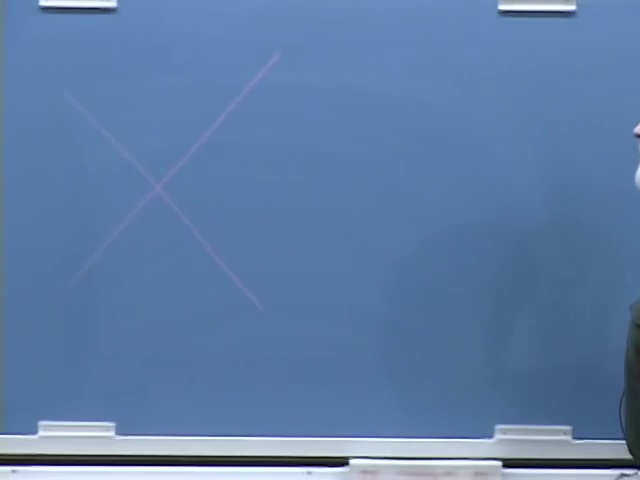
\includegraphics[width=0.68\textwidth]{lecture_09_figure_02.png}
\caption{Nhiệt độ Hawking \(T_H=1/(8\pi M)\) trong đơn vị tự nhiên.}
\lectureframe{00:08:12}
\end{figure}

Lỗ đen càng lớn thì càng lạnh. Bài giảng giải thích điều này bằng cách lần ngược một photon điển hình. Các photon nhiệt có năng lượng đặc trưng \(E_\gamma\sim T_H\). Một photon tới được vô cực với năng lượng cỡ \(M^{-1}\) đã có năng lượng cục bộ lớn hơn nhiều khi nó khởi đầu gần chân trời. Dịch đỏ giữa lớp gần chân trời và vô cực mạnh hơn đối với một lỗ lớn hơn, nên nhiệt độ ở vô cực thấp hơn.

\begin{classroomqa}
\audiencequestion{Nếu thời gian Schwarzschild bị đóng băng tại chân trời, có phải ta nên theo dõi photon ban đầu đã rơi vào và góp phần tạo nên lỗ đen không?\lecturetimestamp{00:04:19}}
\lecturerresponse{Đối với câu hỏi về nhiệt độ, hãy theo các photon phát ra theo hướng ra ngoài. Chúng bắt đầu với tần số cục bộ rất cao, mất năng lượng khi leo ra ngoài, và đến nơi như bức xạ Hawking. Số phận của photon ban đầu rơi vào là một câu hỏi thông tin riêng biệt.}
\end{classroomqa}

\section{Lớp Planck và chân trời kéo giãn}

Quan hệ cục bộ trong Phương trình~\eqref{eq:l09-local-temperature} có thể được tin cậy đến gần tới mức nào? Bài giảng lấy độ dài Planck làm khoảng cách ngắn nhất còn có ý nghĩa trong mô tả bán cổ điển. Điều này gợi ra một lớp mỏng, xấp xỉ một độ dài Planck bên ngoài chân trời toán học, chứa đầy các thăng giáng ở thang Planck. Nó liên tục phát xạ và hấp thụ.

Phần lớn các lượng tử phát ra không thoát được. Chỉ những lượng tử hướng vào một nón rất hẹp ra ngoài mới tránh rơi trở lại. Những lượng tử phóng đi ở các góc thông thường sẽ quay lại chân trời. Các kích thích đi ra và đi vào va chạm, tạo ra các cặp và những hạt khác; theo nghĩa này, mô tả đứng yên chứa một lớp vỏ mỏng gồm vật chất cực nóng.

\begin{figure}[htbp]
\centering
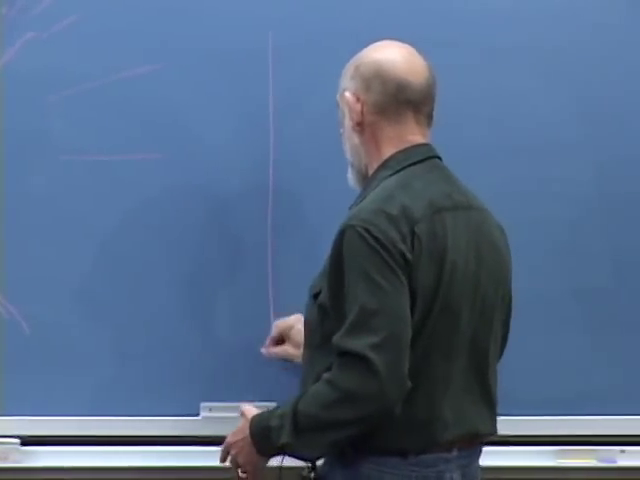
\includegraphics[width=0.74\textwidth]{lecture_09_figure_03.png}
\caption{Nón thoát hẹp của bức xạ gần chân trời. Phần lớn các lượng tử được phát cục bộ quay lại chân trời.}
\lectureframe{00:11:38}
\end{figure}

Có một bức tranh không-thời gian bổ sung. Xa chân trời, một thăng giáng ảo có thể được biểu diễn sơ đồ bằng một vòng kín ngắn: một kích thích hạt-phản hạt xuất hiện rồi biến mất trước khi nó có thể trở thành một trạng thái tiệm cận. Gần chân trời, một thăng giáng có thể bắc qua biên nhân quả. Đối với người quan sát bên ngoài, phần ở ngoài trông như một hạt do chân trời phát ra rồi về sau bị tái hấp thụ. Một phần rất nhỏ thoát ra và trở thành bức xạ Hawking.

\begin{classroomqa}
\audiencequestion{Trong giản đồ miền ngoài, một thăng giáng như vậy có kéo dài từ \(t=-\infty\) đến \(t=+\infty\) không?\lecturetimestamp{00:15:00}}
\lecturerresponse{Chân trời cổ điển chính xác dẫn đến mô tả trông có vẻ kỳ dị đó. Trên thực tế, ta thay nó bằng một chân trời kéo giãn, một siêu mặt kiểu thời gian cách ra ngoài chừng một độ dài Planck. Khi đó, sự phát xạ và tái hấp thụ xảy ra ở những thời gian miền ngoài hữu hạn.}
\end{classroomqa}

\begin{figure}[htbp]
\centering
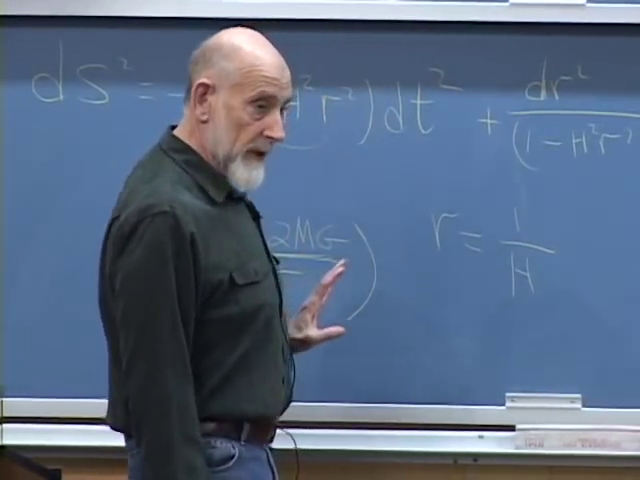
\includegraphics[width=0.72\textwidth]{lecture_09_figure_04.png}
\caption{Chân trời cổ điển và chân trời kéo giãn lân cận được dùng trong mô tả miền ngoài.}
\lectureframe{00:15:52}
\end{figure}

Chân trời kéo giãn không phải là một biên bất biến mới. Nó là một bề mặt hiệu dụng được đặt tại nơi hình học bán cổ điển không còn đáng tin cậy. Các thăng giáng lượng tử của vật chất và của chính hình học làm nhòe vị trí chính xác ở thang Planck. Cách dựng này gói sự bất định đó vào một bề mặt mà trên đó mô tả miền ngoài vẫn hữu hạn.

Không có gì trong lập luận cục bộ này phân biệt việc chân trời thuộc về một lỗ đen hay một vũ trụ đang gia tốc. Đó là chiếc cầu nối sang không gian de Sitter.

\section{Không gian de Sitter trong các tọa độ giãn nở}

Bài giảng chính thức bắt đầu bằng phép cắt phẳng theo không gian của không-thời gian de Sitter,
\begin{equation}
ds^2=-dt^2+e^{2Ht}d\mathbf{x}^2,
\qquad
d\mathbf{x}^2=dx^2+dy^2+dz^2.
\label{eq:l09-flat-slicing}
\end{equation}
Hằng số \(H\) là tốc độ giãn nở de Sitter. Thừa số xuất hiện dưới dạng \(e^{2Ht}\) vì metric đo bình phương khoảng cách; một khoảng tọa độ cố định có độ dài vật lý
\begin{equation}
D(t)=e^{Ht}\lvert\Delta\mathbf{x}\rvert.
\end{equation}

\begin{figure}[htbp]
\centering
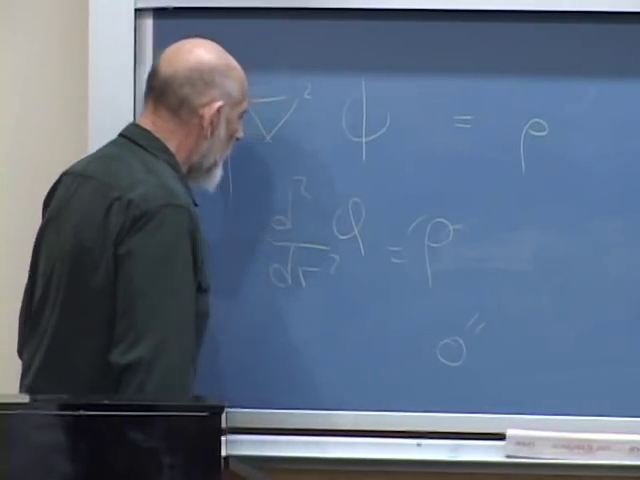
\includegraphics[width=0.78\textwidth]{lecture_09_figure_05.png}
\caption{Metric de Sitter giãn nở theo hàm mũ trong tọa độ phẳng.}
\lectureframe{00:18:50}
\end{figure}

Các tọa độ này làm sự giãn nở trở nên hiển nhiên nhưng đặt vô cực tương lai xa vô hạn lên phía trên trang. Để đưa nó lên bảng, ta đưa vào thời gian bảo giác
\begin{equation}
\eta=-\frac{1}{H}e^{-Ht},
\qquad
-\infty<\eta<0.
\label{eq:l09-conformal-time}
\end{equation}
Khi đó
\begin{equation}
dt=\frac{d\eta}{-H\eta},
\qquad
e^{Ht}=-\frac{1}{H\eta},
\end{equation}
và Phương trình~\eqref{eq:l09-flat-slicing} trở thành
\begin{equation}
ds^2=\frac{1}{H^2\eta^2}
\left(-d\eta^2+d\mathbf{x}^2\right).
\label{eq:l09-conformal-metric}
\end{equation}
Khi \(t\to+\infty\), \(\eta\to0^{-}\). Thời gian riêng vô hạn đã được nén thành đường ngang hữu hạn \(\eta=0\).

\editorialnote{Phép biến đổi thời gian được sửa nhiều lần trong lúc viết trên bảng. Phương trình~\eqref{eq:l09-conformal-time} là dạng nhất quán: thời gian vũ trụ sớm ánh xạ tới \(\eta\to-\infty\), còn vô cực tương lai ánh xạ tới \(\eta\to0^{-}\).}

\begin{figure}[htbp]
\centering
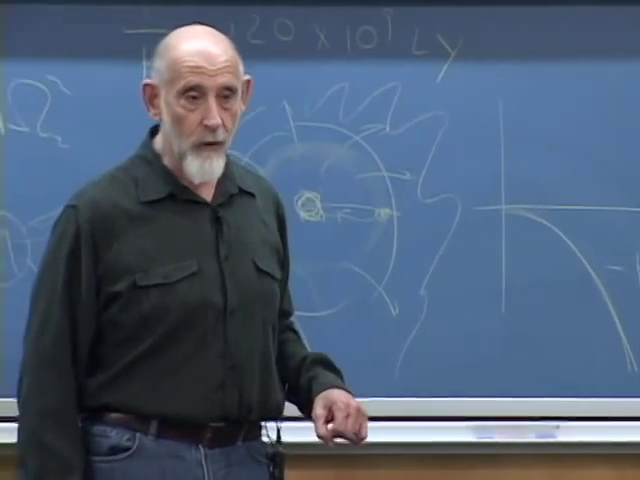
\includegraphics[width=0.82\textwidth]{lecture_09_figure_06.png}
\caption{Phép biến đổi sang thời gian bảo giác và metric phẳng bảo giác.}
\lectureframe{00:21:24}
\end{figure}

Thừa số bảo giác nhân vào cả hạng thời gian lẫn hạng không gian, nên nó không làm thay đổi các phương null. Đối với một tia sáng xuyên tâm,
\begin{equation}
ds^2=0
\quad\Longrightarrow\quad
-d\eta^2+dx^2=0
\quad\Longrightarrow\quad
\frac{dx}{d\eta}=\pm1.
\label{eq:l09-null-rays}
\end{equation}
Vì vậy ánh sáng truyền theo \(45^\circ\) trên giản đồ bảo giác. Đó là lý do phép đổi tọa độ này hữu ích: khả năng tiếp cận nhân quả trở nên nhìn thấy được.

\section{Miền nhân quả của một người quan sát}

Hãy hình dung một người quan sát có đường thế kéo dài trong thời gian riêng vô hạn. Trên giản đồ compact hóa, nó kết thúc tại một điểm trên \(\eta=0\). Mọi tín hiệu mà người quan sát ấy có thể nhận được đều nằm bên trong nón ánh sáng quá khứ của điểm cuối đó. Các sự kiện ở ngoài nón ấy sẽ không bao giờ có thể liên lạc với người quan sát, dù người đó chờ bao lâu đi nữa.

\begin{figure}[htbp]
\centering
\includegraphics[width=0.78\textwidth]{lecture_09_figure_07.png}
\caption{Nón ánh sáng quá khứ giới hạn của một người quan sát trong tọa độ de Sitter bảo giác.}
\lectureframe{00:24:38}
\end{figure}

Một người quan sát thứ hai có một nón khác. Hai miền có thể tiếp cận chồng lấn lên nhau, nhưng không miền nào là toàn bộ không-thời gian. Trong phần còn lại của lập luận, ta nhận quan điểm của người quan sát thứ nhất và gọi nón ánh sáng quá khứ đó là miền nhân quả của người quan sát.

Hình vẽ dường như cho thấy miền ấy co lại về phía tương lai, nhưng độ rộng tọa độ không phải là khoảng cách riêng. Trên một mặt cắt có \(\eta\) không đổi, bình phương khoảng cách vật lý giữa người quan sát tại \(x=0\) và chân trời tại \(x=\Delta x\) là
\begin{equation}
D^2=\frac{(\Delta x)^2}{H^2\eta^2}.
\label{eq:l09-horizon-distance-start}
\end{equation}
Chân trời là một đường null \(45^\circ\) kết thúc tại \(\eta=0\), do đó
\begin{equation}
\Delta x=\lvert\eta\rvert.
\end{equation}
Thay vào ta được
\begin{equation}
D_{\rm hor}^2=\frac{1}{H^2},
\qquad
D_{\rm hor}=\frac{1}{H}.
\label{eq:l09-horizon-radius}
\end{equation}
Độ tách tọa độ co lại, nhưng thừa số bảo giác tăng đúng bằng lượng bù trừ. Bán kính riêng của chân trời là hằng số.

\begin{figure}[htbp]
\centering
\includegraphics[width=0.80\textwidth]{lecture_09_figure_08.png}
\caption{Phép suy ra trên bảng chuyển khoảng tọa độ đang co lại thành khoảng cách riêng cố định \(H^{-1}\).}
\lectureframe{00:28:42}
\end{figure}

\section{Miền tĩnh}

Một bán kính chân trời cố định gợi ý một hệ tọa độ thích nghi với người quan sát ở tâm. Không suy ra phép biến đổi tọa độ, bài giảng viết kết quả:
\begin{equation}
ds^2=
-\left(1-H^2r^2\right)d\tau^2
+\frac{dr^2}{1-H^2r^2}
+r^2d\Omega_2^2.
\label{eq:l09-static-patch}
\end{equation}
Các hệ số phụ thuộc vào \(r\), chứ không phụ thuộc vào \(\tau\). Hệ tọa độ này bao phủ miền tĩnh của người quan sát,
\begin{equation}
0\le r<\frac{1}{H}.
\end{equation}

\begin{figure}[htbp]
\centering
\includegraphics[width=0.88\textwidth]{lecture_09_figure_09.png}
\caption{Metric miền tĩnh de Sitter và sự so sánh của nó với thừa số Schwarzschild.}
\lectureframe{00:34:22}
\end{figure}

Sự giống nhau với Schwarzschild hiện ra ngay lập tức:
\begin{equation}
f_{\rm dS}(r)=1-H^2r^2,
\qquad
f_{\rm Schw}(r)=1-\frac{2G_NM}{r}.
\end{equation}
Trong cả hai trường hợp, chân trời trong tọa độ tĩnh xuất hiện tại nơi \(f(r)=0\). Đối với de Sitter,
\begin{equation}
1-H^2r^2=0
\quad\Longrightarrow\quad
r_H=H^{-1}.
\end{equation}
Hệ tọa độ này kỳ dị tại đó, đúng như tọa độ Schwarzschild kỳ dị tại chân trời lỗ đen. Tuy vậy, các hình học toàn cục khác nhau theo một cách quan trọng. Người quan sát lỗ đen đứng ở bên ngoài và nhìn vào trong; người quan sát de Sitter đứng ở bên trong và nhìn ra ngoài.

\begin{classroomqa}
\audiencequestion{Làm sao hình học có thể tĩnh khi các hạt được buông tự do lại chuyển động xa nhau trong một vũ trụ giãn nở theo hàm mũ?\lecturetimestamp{00:36:06}}
\lecturerresponse{Tĩnh không có nghĩa là mọi hạt đều đứng yên. Nó có nghĩa là các hệ số của metric và kết quả của một thí nghiệm lặp lại không phụ thuộc vào thời điểm bắt đầu. Buông hai hạt bây giờ và chúng gia tốc tách xa nhau; lặp lại cùng thí nghiệm ấy về sau thì cùng chuyển động đó lại xảy ra.}
\end{classroomqa}

\begin{classroomqa}
\audiencequestion{Hai hạt đang tách xa nhau có thấy nhau bị dịch đỏ không?\lecturetimestamp{00:38:34}}
\lecturerresponse{Có. Sự tách xa ngày càng tăng của chúng tạo ra một dịch đỏ tương đối, dù metric thích nghi với người quan sát là độc lập theo thời gian.}
\end{classroomqa}

\section{Nhiệt độ nhìn từ bên trong}

Cấu trúc lân cận chân trời của không gian Schwarzschild và de Sitter là tương đương cục bộ. Vì vậy, chân trời de Sitter phát ra rồi tái hấp thụ các lượng tử nhiệt. Một photon hiếm hoi truyền vào trong tới người quan sát ở tâm, mất năng lượng khi leo ngược thế của miền tĩnh. Nhiệt độ Gibbons--Hawking đo tại tâm là
\begin{equation}
T_{\rm dS}=\frac{H}{2\pi}
\label{eq:l09-de-sitter-temperature}
\end{equation}
trong đơn vị tự nhiên. Một nhiệt kế đứng yên tại bán kính \(r\) đo được giá trị bị dịch đỏ theo Tolman
\begin{equation}
T_{\rm local}(r)=
\frac{T_{\rm dS}}{\sqrt{1-H^2r^2}},
\label{eq:l09-tolman}
\end{equation}
đại lượng này phân kỳ khi \(r\to H^{-1}\) và ở gần chân trời thì rút gọn về Phương trình~\eqref{eq:l09-local-temperature}.

\editorialnote{Bài giảng suy ra thang độ lớn từ khoảng cách tới chân trời và độ dịch đỏ thay vì viết tường minh các Phương trình~\eqref{eq:l09-de-sitter-temperature} và \eqref{eq:l09-tolman}. Ở đây nêu ra cách chuẩn hóa tiêu chuẩn của lập luận đó.}

Đối với gia tốc muộn quan sát được, bài giảng dùng ước lượng chu kỳ
\begin{equation}
H^{-1}\sim 20\times10^9\ {\rm light\ years}.
\label{eq:l09-lecture-horizon-estimate}
\end{equation}
Khi đó, một photon chân trời điển hình có bước sóng cỡ hàng tỉ năm ánh sáng. Đây không phải bức xạ nền vi sóng; nó lạnh hơn rất nhiều.

Thí nghiệm tưởng tượng mang tính thao tác là một cần câu ở quy mô vũ trụ học. Alice ở lại tại \(r=0\), gắn một nhiệt kế vào một sợi dây rất dài đồng thời truyền dữ liệu, rồi để lực đẩy vũ trụ đưa thiết bị ra ngoài. Cô dừng nó ngay trước chân trời, chờ tín hiệu quay về, và thấy một nhiệt độ cục bộ lớn. Nhiệt kế đặt cạnh cô ở tâm chỉ giá trị rất nhỏ \(H/(2\pi)\). Cùng một chân trời cho ra cả hai số đo vì chúng được thực hiện tại những thế hấp dẫn khác nhau.

\section{Vượt qua chân trời}

Mô tả cổ điển từ bên ngoài giống với câu chuyện hố đen quen thuộc. Bob ở tâm nhìn Alice lùi xa dần. Tín hiệu của cô bị dịch đỏ ngày càng mạnh và đến ngày càng chậm; cô dường như bị ép dẹt lên chân trời rồi cuối cùng mờ hẳn đi. Một người du hành đến sau, Jane, hiện ra như một lớp khác còn mỏng hơn trong một chồng trầm tích gần biên.

\begin{classroomqa}
\audiencequestion{Từ quan điểm của chúng ta, các vật thể có bao giờ đi qua chân trời vũ trụ không?\lecturetimestamp{00:45:30}}
\lecturerresponse{Không, trong mô tả cổ điển của người quan sát tĩnh. Tín hiệu của chúng bị dịch đỏ và mờ dần trong khi vị trí biểu kiến của chúng tiến sát chân trời. Tuy nhiên, trong mô tả rơi tự do của chính chúng, chúng đi qua mà không gặp một bề mặt kỳ dị cục bộ nào.}
\end{classroomqa}

\begin{classroomqa}
\audiencequestion{Chân trời chỉ nóng đối với các quan sát viên ở gần mà không băng qua nó thôi sao? Một người quan sát rơi vào không bị nấu chín chỉ vì đi qua nó, đúng không?\lecturetimestamp{00:48:27}}
\lecturerresponse{Alice đi qua trơn tru trong hệ quy chiếu riêng của cô. Nhiệt độ cực cao thuộc về mô tả đứng yên. Nếu Bob cứ khăng khăng phân giải Alice ngày càng sát chân trời, ông phải chiếu sáng cô bằng những bước sóng ngày càng ngắn. Khi đó, kính hiển vi Heisenberg trong nỗ lực ấy sẽ nạp vào đủ năng lượng để nấu chín chính thứ nó đang cố quan sát.}
\end{classroomqa}

Đây không phải là một mâu thuẫn giữa hai sự kiện cục bộ. Người quan sát đứng yên và người rơi vào dùng những phép đo khác nhau một cách căn bản. Tính bổ sung chân trời đặt câu hỏi làm thế nào cả hai mô tả đều có thể đúng mà không cho phép một người quan sát nào trực tiếp so sánh thông tin trùng lặp.

\section{Mô hình Newton của lực đẩy chân không}

Đến đây một sinh viên hỏi điều gì đóng vai trò thay cho giếng thế hấp dẫn của hố đen. Susskind trả lời bằng cách xây dựng một mô hình Newton. Gọi \(\phi\) là thế hấp dẫn, khi đó gia tốc của một hạt thử là
\begin{equation}
\mathbf{a}=-\boldsymbol{\nabla}\phi.
\end{equation}
Đối với vật chất thông thường không tương đối tính, phương trình Poisson là
\begin{equation}
\nabla^2\phi=4\pi G_N\rho.
\label{eq:l09-poisson}
\end{equation}

\begin{classroomqa}
\audiencequestion{Nếu các hiệu ứng của hố đen đến từ giếng thế hấp dẫn của nó, thì nguồn tương ứng trong không gian de Sitter là gì?\lecturetimestamp{00:49:36}}
\lecturerresponse{Chính năng lượng chân không cung cấp một nguồn hấp dẫn đồng nhất theo không gian. Trong mô tả Newton, nó tạo ra một thế bậc hai chứ không phải một giếng thế \(1/r\).}
\end{classroomqa}

\begin{figure}[htbp]
\centering
\includegraphics[width=0.78\textwidth]{lecture_09_figure_10.png}
\caption{Phương trình Poisson và dạng đạo hàm bậc hai theo bán kính mang tính sơ đồ trong bài giảng.}
\lectureframe{00:51:38}
\end{figure}

Trên bảng, người giảng lược bỏ hệ số chuẩn hóa, các hạng do độ đo cầu, áp suất, và lúc đầu thậm chí cả dấu tổng thể, khiến bài toán rút xuống còn
\begin{equation}
\frac{d^2\phi}{dr^2}\sim H^2.
\end{equation}
Suy luận cốt lõi là một nguồn hằng cho ra một hàm bậc hai. Với dấu cần có cho lực đẩy de Sitter,
\begin{equation}
\phi_{\rm dS}(r)=-\frac{1}{2}H^2r^2,
\qquad
a_r=-\frac{d\phi_{\rm dS}}{dr}=H^2r.
\label{eq:l09-de-sitter-potential}
\end{equation}
Gia tốc hướng ra ngoài và tăng tuyến tính theo khoảng cách. Giải \(\ddot r=H^2r\) thu được
\begin{equation}
r(\tau)=A e^{H\tau}+B e^{-H\tau},
\end{equation}
nên nhánh tăng tái tạo sự tách xa theo hàm mũ.

\begin{figure}[htbp]
\centering
\includegraphics[width=0.76\textwidth]{lecture_09_figure_11.png}
\caption{Phương trình nguồn đồng nhất và thế de Sitter bậc hai.}
\lectureframe{00:53:32}
\end{figure}

\editorialnote{Trong thuyết tương đối rộng, gia tốc trong gần đúng trường yếu của một lưu chất đồng nhất phụ thuộc vào \(\rho+3p\), chứ không chỉ vào \(\rho\). Năng lượng chân không có \(p=-\rho\), nên \(\rho+3p=-2\rho\) và gia tốc là đẩy ra. Phương trình~\eqref{eq:l09-de-sitter-potential} là kết quả de Sitter với chuẩn hóa đúng; phép tính trên bảng cố ý chỉ theo dõi phụ thuộc bậc hai và dấu.}

Đặt một khối lượng thông thường \(M\) tại tâm. Thế định tính khi đó trở thành
\begin{equation}
\phi(r)=-\frac{G_NM}{r}-\frac{1}{2}H^2r^2,
\label{eq:l09-combined-potential}
\end{equation}
và gia tốc theo bán kính là
\begin{equation}
a_r=-\frac{G_NM}{r^2}+H^2r.
\end{equation}
Khi \(r\) nhỏ, lực hút cục bộ thắng; khi \(r\) lớn, lực đẩy chân không thắng. Sự cân bằng của chúng xảy ra tại
\begin{equation}
r_\ast=\left(\frac{G_NM}{H^2}\right)^{1/3}.
\label{eq:l09-turnaround}
\end{equation}
Đây là phiên bản gọn gàng của cực đại thế trong bài giảng. Nó giải thích về mặt định tính vì sao các hệ bị liên kết hấp dẫn ở gần có thể vẫn ở cùng nhau trong khi những thiên hà đủ xa thì gia tốc rời xa nhau.

\begin{figure}[htbp]
\centering
\includegraphics[width=0.78\textwidth]{lecture_09_figure_12.png}
\caption{Lực hút thông thường \(1/r\) kết hợp với thế de Sitter bậc hai lật ngược.}
\lectureframe{00:58:20}
\end{figure}

\begin{classroomqa}
\audiencequestion{Các lực thông thường còn quan trọng không, hay lực đẩy chân không rốt cuộc sẽ xé toạc mọi hòn đảo vật chất?\lecturetimestamp{00:57:29}}
\lecturerresponse{Mọi lực đều phải được tính đến. Trên những thang đủ nhỏ, liên kết điện từ và hấp dẫn cục bộ chi phối. Lực đẩy chân không chỉ trở nên quan trọng trên những khoảng cách khổng lồ được đặt bởi \(H^{-1}\) và bởi thang cân bằng thích hợp với khối lượng liên kết.}
\end{classroomqa}

\section{Một nguồn, nhiều tên gọi}

Phần thảo luận giờ tạm dừng ở thuật ngữ. Năng lượng chân không, hằng số vũ trụ và năng lượng tối không phải là ba thành phần cộng gộp trong mô hình đang dùng. Chúng là ba cách mô tả cùng một nguồn \(w=-1\). Ta có thể nói tới một hạng hằng trong phương trình Einstein, một mật độ năng lượng chân không bất biến Lorentz, hoặc thành phần thúc đẩy gia tốc ở thời muộn.

\begin{classroomqa}
\audiencequestion{Nguồn Newton đồng nhất và năng lượng chân không lượng tử có cùng hiện diện như các hiệu ứng tách biệt không?\lecturetimestamp{00:59:14}}
\lecturerresponse{Không. Mật độ đồng nhất là mô hình Newton của cùng một nguồn đó. Năng lượng chân không, hằng số vũ trụ và, trong bài giảng này, năng lượng tối đều chỉ một thành phần vật lý.}
\end{classroomqa}

\begin{classroomqa}
\audiencequestion{Vậy cùng một hiện tượng có một mô tả cổ điển và một mô tả lượng tử phải không?\lecturetimestamp{01:00:32}}
\lecturerresponse{Nguồn gốc vi mô của nó có thể là cơ học lượng tử, cũng như một phần khối lượng của electron có nguồn gốc lượng tử. Một khi mật độ năng lượng hiệu dụng đã được biết, nó đi vào các phương trình hấp dẫn cổ điển như một nguồn thông thường. Chúng ta không biết nguồn gốc tối hậu của giá trị quan sát được.}
\end{classroomqa}

Trong đơn vị Planck, mật độ năng lượng chân không quan sát được là cực kỳ nhỏ,
\begin{equation}
\rho_\Lambda\sim10^{-123}\rho_{\rm Pl},
\label{eq:l09-planck-smallness}
\end{equation}
tùy theo quy ước dùng cho mật độ Planck. Con số nhỏ đó chính là bài toán hằng số vũ trụ. Đó cũng là lý do chân trời lại lớn đến vậy: trong bốn chiều,
\begin{equation}
H^2=\frac{8\pi G_N}{3}\rho_\Lambda,
\qquad
r_H=H^{-1}.
\end{equation}
Nếu \(H\) lớn hơn, chân trời sẽ nhỏ hơn, nhiệt độ de Sitter tại tâm sẽ cao hơn, và gia tốc đẩy \(H^2r\) sẽ mạnh hơn.

\begin{classroomqa}
\audiencequestion{Hằng số vũ trụ rất nhỏ có liên hệ với hằng số Planck và các dao động lượng tử không?\lecturetimestamp{01:03:27}}
\lecturerresponse{Phép so sánh gọn gàng nhất dùng các đơn vị Planck không thứ nguyên, trong đó \(G_N=\hbar=c=1\). Trong các đơn vị ấy, mật độ chân không thấp hơn mật độ Planck tự nhiên khoảng \(123\) bậc độ lớn. Giải thích sự phân cấp đó là một trong những câu đố trung tâm của vật lý cơ bản.}
\end{classroomqa}

\begin{classroomqa}
\audiencequestion{Năng lượng chân không có nhất thiết phải là một hằng số vũ trụ đúng nghĩa không đổi không? Thành phần gây gia tốc có thể giảm đi và cuối cùng về không không?\lecturetimestamp{01:04:52}}
\lecturerresponse{Đó là một khả năng thay thế hợp logic: một trường năng lượng tối động lực học có thể biến thiên theo thời gian. Bài giảng dùng trường hợp hằng vì những quan sát hiện có vào thời điểm đó ngày càng ủng hộ hành vi gần với một hằng số vũ trụ, chứ không phải vì mọi phương án thay thế đã được chứng minh là bất khả.}
\end{classroomqa}

\section{Thiên văn học trong tương lai xa}

Trong một vũ trụ tiệm cận de Sitter, các cấu trúc không bị liên kết hấp dẫn rốt cuộc sẽ đi qua chân trời của người quan sát. Phông vi sóng vũ trụ bị dịch đỏ xuống dưới ngưỡng phát hiện. Các thiên hà xa biến mất. Một nhà thiên văn còn lại có thể chỉ nhìn thấy một hòn đảo hấp dẫn địa phương đã sáp nhập nằm trong một vùng còn lại thì tối đen.

\begin{classroomqa}
\audiencequestion{Không có kính thiên văn, liệu có ai thậm chí nhận ra rằng các thiên hà xa đã biến mất không?\lecturetimestamp{01:06:17}}
\lecturerresponse{Có lẽ là không. Vấn đề nghiêm trọng hơn còn sâu hơn: ngay cả với các thiết bị tiên tiến, những người quan sát tương lai có thể thiếu các chỉ dấu xa và phông vi sóng mà từ đó ngày nay chúng ta suy ra sự giãn nở.}
\end{classroomqa}

Khi đó, bức tranh vũ trụ-đảo cũ có thể trở nên rất thuyết phục. Nghịch lý Olbers sẽ không buộc ta đi đến một kết luận khác, vì nó giả sử có một quần thể vô hạn, tĩnh và đồng đều của các nguồn sáng; người quan sát tương lai sẽ chỉ thấy các ngôi sao hữu hạn của hòn đảo địa phương. Năng lượng tối không liên tục tạo ra các thiên hà thay thế từ không gian trống rỗng.

Chân trời trong không gian de Sitter chính xác không co lại quanh thiên hà địa phương. Bán kính vật lý của nó vẫn là \(H^{-1}\), lớn hơn một thiên hà rất nhiều. Điều biến mất là vật chất không bị liên kết bị mang ra ngoài biên nhân quả cố định đó.

\begin{classroomqa}
\audiencequestion{Các ngôi sao bị bắn văng khỏi thiên hà có thể làm các vật thử để phát hiện hình học quy mô lớn không?\lecturetimestamp{01:11:25}}
\lecturerresponse{Trong một thời gian thì có. Các vật bị văng ra và các tín hiệu ánh sáng có đường cơ sở dài có thể thăm dò hình học. Nhưng hiệu ứng chỉ trở nên đáng kể trên những khoảng cách cỡ một phần đáng kể của một tỉ năm ánh sáng, nên thí nghiệm sẽ mất thời gian vũ trụ học.}
\end{classroomqa}

\begin{classroomqa}
\audiencequestion{Làm sao ta biết rằng một chân trời xa chưa che khuất phần lớn vũ trụ khỏi chúng ta?\lecturetimestamp{01:11:45}}
\lecturerresponse{Chúng ta đã nhìn thấy đủ nhiều thiên hà, độ dịch đỏ và bức xạ nền để đo sự giãn nở và phục dựng hình học quy mô lớn. Những người quan sát tương lai bị tước mất các chỉ dấu ấy sẽ đối diện một bài toán suy luận khó hơn nhiều.}
\end{classroomqa}

\begin{classroomqa}
\audiencequestion{Nếu chân trời nằm ngay bên ngoài Andromeda, sự hiện diện của nó có hiển nhiên không?\lecturetimestamp{01:12:19}}
\lecturerresponse{Có. Một chân trời nhỏ như vậy sẽ đòi hỏi \(H\) lớn hơn nhiều, và lực đẩy do đó sinh ra sẽ làm biến đổi mạnh chuyển động của Andromeda. Thay vào đó, giá trị đo được đặt chân trời tiệm cận ở một thang lớn hơn rất nhiều.}
\end{classroomqa}

\begin{classroomqa}
\audiencequestion{Những vụ nổ lớn mới có thể đang xảy ra bên ngoài chân trời của chúng ta không?\lecturetimestamp{01:13:25}}
\lecturerresponse{Các sự kiện bên ngoài chân trời là không thể nhìn thấy đối với chúng ta hoặc các hậu duệ của chúng ta. Một khả năng liên quan nhưng chính xác hơn, sự tạo mầm bong bóng trong lạm phát vĩnh cửu, sẽ được giới thiệu về sau trong bài giảng.}
\end{classroomqa}

Với tên lửa, đồng hồ và vài tỉ năm, những người quan sát tương lai có thể gửi các nhà thám hiểm đi qua một phần lớn của miền này và phục dựng metric của nó. Tuy nhiên, trên các thang thời gian phòng thí nghiệm hay văn minh thông thường, hiệu ứng ấy gần như ngoài tầm tiếp cận. Sự phân biệt này sửa lại khẳng định quá mạnh rằng sự giãn nở sẽ không thể được khám phá: về mặt thao tác nó rất xa tầm với, chứ không bị cấm về nguyên tắc.

\begin{classroomqa}
\audiencequestion{Liệu các nhà thám hiểm tương lai có thể xác định hình học sớm hơn rất nhiều so với việc chờ một lần hồi quy nhiệt hay không?\lecturetimestamp{01:21:40}}
\lecturerresponse{Chắc chắn là có. Một lần hồi quy không phải là phép đo được đề xuất. Các nhà thám hiểm trao đổi tín hiệu ánh sáng trên những đường cơ sở dài hàng tỷ năm ánh sáng có thể lập bản đồ vùng tĩnh trên một thang thời gian ngắn hơn rất nhiều, dù vẫn còn ở quy mô vũ trụ học.}
\end{classroomqa}

\begin{classroomqa}
\audiencequestion{Liệu dịch đỏ có xóa sạch mọi thông tin mà các nhà thám hiểm như vậy gửi về không?\lecturetimestamp{01:23:24}}
\lecturerresponse{Không, nếu họ thăm dò các thang nằm sâu bên trong chân trời. Một đường cơ sở cỡ một tỷ năm ánh sáng đã nhạy với sự giãn nở, trong khi chỉ tạo ra một dịch đỏ vừa phải. Thí nghiệm chủ yếu bị giới hạn bởi thời lượng khổng lồ của nó.}
\end{classroomqa}

\section{Entropy hữu hạn và sự hồi quy}

Vùng tĩnh không rỗng theo nghĩa nhiệt động học. Chân trời của nó có diện tích
\begin{equation}
A_H=4\pi H^{-2},
\end{equation}
nhiệt độ là \(T_{\rm dS}=H/(2\pi)\), và entropy
\begin{equation}
S_{\rm dS}=\frac{A_H}{4G_N}
=\frac{\pi}{G_NH^2}
\label{eq:l09-de-sitter-entropy}
\end{equation}
trong các đơn vị \(\hbar=c=k_B=1\). Entropy là hữu hạn. Vì thế, với sự dè dặt thích hợp, ta có thể hình dung vùng tĩnh như một khoang nhiệt có entropy hữu hạn, mà trong mô tả dừng thì các kích thích của nó tập trung gần chân trời.

Một hộp khí thông thường ở trạng thái cân bằng trông không có đặc trưng gì trên các thang thời gian ngắn, nhưng cơ học thống kê không cấm các thăng giáng. Nếu một trạng thái vĩ mô có độ hụt entropy \(\Delta S\) so với cân bằng, thì xác suất của nó xấp xỉ là
\begin{equation}
P\sim e^{-\Delta S}.
\label{eq:l09-fluctuation-probability}
\end{equation}
Thời gian chờ tương ứng tăng theo
\begin{equation}
t\sim t_0 e^{\Delta S}.
\end{equation}
Đối với một hệ hữu hạn, thời gian để quay lại một trạng thái gần tùy ý với một trạng thái trước đó là thời gian hồi quy Poincaré,
\begin{equation}
t_{\rm rec}\sim H^{-1}e^{S_{\rm dS}}.
\label{eq:l09-recurrence}
\end{equation}
Vì \(S_{\rm dS}\) đối với chân trời của chúng ta có bậc cỡ \(10^{120}\), bài giảng tóm tắt thang này là \(e^{10^{120}}\). Hệ số tiền nhân được đo bằng năm, thời gian Hubble hay các đơn vị vi mô đều không quan trọng so với hàm mũ kép.

\begin{figure}[htbp]
\centering
\includegraphics[width=0.76\textwidth]{lecture_09_figure_13.png}
\caption{Phần thảo luận về sự hồi quy, với thang thời gian chờ theo hàm mũ khổng lồ trên bảng.}
\lectureframe{01:16:24}
\end{figure}

Trước một lần hồi quy như thế, các thăng giáng nhỏ hơn phổ biến hơn rất nhiều. Các phân tử trong một căn phòng có thể đều tụ lại ở một góc; một xoáy phức tạp có thể thoáng hình thành; trong thứ bậc đùa vui của bài giảng, chuyển động nhiệt có thể lắp ghép nên một con voi. Độ hụt entropy cần thiết càng nhỏ, thăng giáng càng ít tốn kém.

\begin{classroomqa}
\audiencequestion{Liệu các hồi quy Poincaré có phải riêng là hệ quả của cơ học lượng tử không?\lecturetimestamp{01:25:44}}
\lecturerresponse{Không. Sự hồi quy và các thăng giáng hiếm đã xuất hiện ngay trong cơ học thống kê cổ điển. Việc áp dụng chúng vào không gian de Sitter sử dụng khuôn khổ vật lý hiện nay của chúng ta, khuôn khổ ấy có thể một ngày nào đó sẽ được sửa đổi, nhưng nhiệt động học và suy luận thống kê thuộc số những cấu trúc vững chắc nhất mà chúng ta biết.}
\end{classroomqa}

Bản thân ý nghĩa của xác suất có thể sẽ được hiểu sâu hơn trong một lý thuyết tương lai. Susskind không phủ nhận điều đó. Điểm ông muốn nêu hẹp hơn: từ bỏ cơ học thống kê chỉ vì những hệ quả ở thời gian dài của nó nghe kỳ lạ sẽ là vứt bỏ một trong những nguyên lý tổ chức của vật lý đã được kiểm nghiệm kỹ nhất.

\section{Não Boltzmann và các quan sát viên điển hình}

Giả sử một thăng giáng nhiệt tạo ra trọn vẹn một trạng thái giống Vụ Nổ Lớn. Điều đó đòi hỏi một sự giảm entropy khổng lồ. Một thăng giáng tạo ra một hệ hành tinh thì ít tốn kém hơn; một Trái Đất vốn đã ấm còn ít tốn kém hơn nữa. Nếu điều kiện duy nhất là có một quan sát viên, thì thăng giáng ít tốn kém nhất có thể chỉ tạo ra một bộ não đang hoạt động hoàn chỉnh kèm theo những ký ức bề ngoài có vẻ sẵn có. Một quan sát viên giả thuyết như vậy được gọi là một não Boltzmann.

Vấn đề không phải là liệu một thăng giáng kỳ quái nào đó có khả hữu về mặt lôgic hay không. Vấn đề là liệu một mô hình vũ trụ học có tiên đoán rằng hầu như mọi quan sát viên đều là một thăng giáng như thế hay không. Ta suy luận từ các quan sát của mình bằng cách giả sử rằng mình không dị thường đến mức khó tin. Một lý thuyết trong đó các quan sát viên thông thường với lịch sử vũ trụ mạch lạc bị các bộ não nhiệt cô lập áp đảo theo hàm mũ về số lượng sẽ phá hỏng suy luận ấy.

Vì vậy, bài toán não Boltzmann là tên gọi của một phép kiểm tra tính nhất quán định lượng. Người ta so sánh độ phong phú kỳ vọng của các quan sát viên thông thường với độ phong phú của các quan sát viên được sinh ra từ thăng giáng. Nếu loại sau chiếm ưu thế, thì hoặc chân không phải phân rã trước khi chúng tăng sinh, hoặc phải thay đổi độ đo, hoặc phải xem xét lại các giả định vũ trụ học.

Một câu hỏi trước đó về mối liên hệ tử ngoại--hồng ngoại được hoãn lại một cách minh thị. Lập luận về sự hồi quy không phụ thuộc vào việc giải quyết vấn đề tách biệt đó.

\section{Lạm phát vĩnh cửu và các vũ trụ bong bóng}

Tiếp theo, bài giảng giới thiệu, mà không cố gắng đưa ra một suy dẫn đầy đủ, một bài toán xác suất thứ hai. Một trạng thái chân không de Sitter giả bền có thể tạo mầm một bong bóng mà trong đó năng lượng chân không thấp hơn. Vách bong bóng giãn ra, và phần bên trong có thể phát triển thành một vũ trụ Friedmann--Robertson--Walker mở. Trong khi đó, miền đang lạm phát xung quanh tiếp tục giãn nở và tạo mầm thêm nhiều bong bóng.

\begin{figure}[htbp]
\centering
\includegraphics[width=0.74\textwidth]{lecture_09_figure_14.png}
\caption{Một bong bóng có năng lượng chân không thấp hơn được vẽ bên trong một nền de Sitter đang lạm phát.}
\lectureframe{01:29:38}
\end{figure}

Đặc trưng then chốt là sự tăng trưởng số lượng theo hàm mũ. Thể tích vật lý mới được tạo ra nhanh hơn tốc độ các bong bóng lấy đi nó, nên số miền bong bóng tăng lên không bị chặn. Các bong bóng khác nhau có thể lắng vào những trạng thái năng lượng thấp khác nhau và vì thế biểu lộ những vật lý hiệu dụng khác nhau.

Để phơi bày khó khăn thống kê, trước hết Susskind rời khỏi vũ trụ học và xét một dân số loài người tăng theo hàm mũ với nguồn lực hữu hạn nhưng chưa biết. Giả sử các quan sát viên là điển hình trong số tất cả những người từng sống. Nếu dân số tăng gấp đôi sau mỗi thế hệ rồi kết thúc, thì một nửa mọi người sống ở thế hệ cuối, ba phần tư sống ở hai thế hệ cuối, và bảy phần tám sống ở ba thế hệ cuối:
\begin{equation}
f_n=1-2^{-n}.
\label{eq:l09-last-generations}
\end{equation}
Khi đó, tính điển hình sẽ đặt chúng ta ở gần cuối một cách đáng ngại, mặc dù ta không biết gì về tổng nguồn lực. Điều này không được đưa ra như một dự đoán đáng tin cậy về sự tuyệt chủng của loài người. Nó là một lời cảnh báo rằng tăng trưởng theo hàm mũ khiến việc đếm bị chi phối bởi mốc cắt.

Ví dụ tung đồng xu phát biểu giả định điển hình thông thường một cách sáng sủa hơn. Nếu nhiều người làm thí nghiệm, mỗi người tung một đồng xu cân bằng \(N\) lần, thì đa số áp đảo sẽ thu được
\begin{equation}
n_H=\frac{N}{2}+O(\sqrt{N}).
\end{equation}
Một quan sát viên có kết quả cực đoan trước tiên nên nghi ngờ mô hình sai hoặc đồng xu có vấn đề, thay vì giả định vô bằng cớ rằng mình nằm trong một đuôi phân bố hiếm đến khó tin. Xác suất vũ trụ học dùng cùng trực giác về tính điển hình ấy, nhưng trong một quần thể vô hạn nó cần một cách đếm được xác định rõ.

\section{Biên của Escher và bài toán độ đo}

Phép loại suy hình học của Susskind là tác phẩm của M.\ C.\ Escher, \emph{Circle Limit IV}, một chiếc đĩa được lát kín bởi các thiên thần và ác quỷ trông nhỏ dần về phía biên. Trong hình học hyperbol được bức vẽ biểu diễn, các hình đó là tương đương; kích thước Euclid biểu kiến của chúng chỉ thay đổi vì phép chiếu.

\begin{figure}[htbp]
\centering
\includegraphics[width=0.76\textwidth]{lecture_09_figure_15.png}
\caption{Hình thay thế trên bảng cho các hình của Escher tăng sinh theo hàm mũ gần một biên tròn.}
\lectureframe{01:37:54}
\end{figure}

Hãy tưởng tượng Escher có thời gian, mực và sự kiên nhẫn đều hữu hạn. Gần mép, cuối cùng ông dừng lại, có lẽ để một số hình còn dang dở. Vì số lượng hình tăng theo hàm mũ theo bán kính hyperbol, một lớp ngoài hữu hạn chứa một phần cỡ đơn vị cố định của toàn bộ các hình đã vẽ. Xấp xỉ một nửa có thể nằm trong lớp cuối cùng, bất kể mốc cắt được dời ra xa đến đâu.

Bây giờ hãy hỏi tỉ số giữa thiên thần và ác quỷ. Trong mẫu hình vô hạn lý tưởng, tính đối xứng gợi ý sự bằng nhau một đối một. Tuy nhiên, trong bất kỳ phép đếm hữu hạn nào, một đường biên hơi khác đi cũng có thể bao hàm nhiều hơn hẳn các hình thuộc một loại. Vì phần lớn phép đếm nằm gần đường biên, một biến dạng nhỏ của đường biên ấy tạo ra một thay đổi cỡ đơn vị trong đáp án.

\begin{figure}[htbp]
\centering
\includegraphics[width=0.76\textwidth]{lecture_09_figure_16.png}
\caption{Biên cắt cụt chi phối phép đếm trong một mẫu hình tăng trưởng theo hàm mũ.}
\lectureframe{01:43:06}
\end{figure}

Sự mơ hồ tương tự cũng xuất hiện trong lạm phát vĩnh cửu. Hãy đếm các vũ trụ bong bóng xanh và hồng trước một mốc cắt theo thời gian nào đó, rồi đẩy mốc cắt ấy về muộn hơn. Cả hai phép đếm đều phân kỳ, và tỉ số của chúng có thể phụ thuộc nhạy vào việc \emph{thời gian} có nghĩa là gì và mặt cắt được vẽ như thế nào. Một độ đo xác suất là một quy tắc điều chỉnh quần thể vô hạn và rút ra các xác suất tương đối. Việc những quy tắc khả dĩ khác nhau không cho cùng một kết quả chính là bài toán độ đo.

\begin{classroomqa}
\audiencequestion{Có quan hệ nào giữa bài toán cắt cụt này và tái chuẩn hóa không?\lecturetimestamp{01:45:43}}
\lecturerresponse{Có một phép loại suy. Trong lý thuyết trường lượng tử, người ta đưa vào một mạng hoặc một cắt cụt tử ngoại, tinh chỉnh nó, và tìm những đại lượng không nhạy với các chi tiết ở rìa của bộ điều chuẩn. Các nhà vũ trụ học hy vọng có được một sự rút trích từ lạm phát vĩnh cửu cũng vững chắc như vậy, nhưng trong khuôn khổ đang được bàn ở đây vẫn chưa có một quy tắc có sức quyết định tương đương.}
\end{classroomqa}

Không nên đẩy phép loại suy này đi quá xa. Tái chuẩn hóa thành công khi một dòng chảy được kiểm soát xác định được các đại lượng quan sát được độc lập với bộ điều chuẩn. Bài toán độ đo chính là ở chỗ các câu hỏi bất biến tương tự và thủ tục lấy giới hạn vẫn còn chưa rõ. Nói rằng có thể ta đang đặt sai câu hỏi không phải là một lời giải cho đến khi câu hỏi đúng được cung cấp.

\begin{classroomqa}
\audiencequestion{Bức tranh bong bóng này có phải là cùng hiện tượng với lạm phát trong vũ trụ sơ khai của chúng ta không?\lecturetimestamp{01:48:19}}
\lecturerresponse{Nó có liên hệ rất chặt chẽ. Trong lạm phát vĩnh cửu, nền mẹ tiếp tục lạm phát trong khi phần bên trong cục bộ của các bong bóng trải qua tiến hóa vũ trụ học riêng của chúng. Vũ trụ quan sát được của chúng ta có thể nằm bên trong một miền như vậy.}
\end{classroomqa}

\section{Liệu có thể quan sát được các va chạm bong bóng không?}

Khi gặp nhau, hai bong bóng không đơn giản cộng năng lượng chân không của chúng lại. Một vách miền ngăn cách các miền có trạng thái chân không khác nhau, và hình học của vách quyết định mỗi phía có thể quan sát được gì. Tùy theo vị trí của va chạm so với nón ánh sáng quá khứ của chúng ta, dấu vết của nó có thể bị che khuất hoặc có thể nhìn thấy.

\begin{classroomqa}
\audiencequestion{Điều gì xảy ra khi hai bong bóng chân không va chạm?\lecturetimestamp{01:52:07}}
\lecturerresponse{Va chạm tạo ra một hình học vách miền mà hành vi của nó phụ thuộc vào hai chân không và vào sức căng của vách. Trong những hoàn cảnh nhân quả thuận lợi, nhiễu loạn có thể đi vào miền quan sát được của chúng ta và để lại một dấu hiệu bất đẳng hướng.}
\end{classroomqa}

Bài giảng bàn đến một vùng lạnh trong phông vi sóng vũ trụ như một ứng viên khả dĩ và chỉ ra phân cực quanh một đặc trưng hình tròn như một dấu hiệu phân biệt. Điều này được trình bày có chủ ý như một khả năng, chứ không phải một phát hiện. Một dấu hiệu va chạm đủ sức thuyết phục sẽ mang tính cách mạng vì nó sẽ cung cấp bằng chứng trực tiếp về các miền bong bóng lân cận và khiến bài toán độ đo trở nên cấp bách về mặt thực nghiệm.

\begin{figure}[htbp]
\centering
\includegraphics[width=0.70\textwidth]{lecture_09_figure_17.png}
\caption{Một đặc trưng tròn trên bầu trời và mẫu phân cực khả dĩ của nó trong phần thảo luận về va chạm bong bóng.}
\lectureframe{01:50:22}
\end{figure}

\editorialnote{Phần thảo luận về điểm lạnh ghi lại tình trạng quan sát và các đề xuất vào thời điểm của bài giảng. Bản thân một dị thường nhiệt độ không phải là bằng chứng của va chạm bong bóng; cần có một dấu hiệu chi tiết và tương quan.}

\begin{classroomqa}
\audiencequestion{Các bong bóng có phải là bốn chiều không, và phần bên trong của chúng có độ cong không gian nào?\lecturetimestamp{01:53:37}}
\lecturerresponse{Chúng là các miền không-thời gian, không phải các bong bóng xà phòng ba chiều tiến hóa trong một thời gian bên ngoài. Phần bên trong của chúng thường là các vũ trụ FRW mở với độ cong không gian âm. Một va chạm làm nhiễu loạn hình học đó nhưng không đơn giản biến độ cong âm thành độ cong dương.}
\end{classroomqa}

\section{Lý thuyết dây xác lập và không xác lập điều gì}

Phần thảo luận cuối cùng mở đầu bằng lời mời gán một xác suất cho việc lý thuyết dây là đúng. Susskind từ chối đưa ra con số ấy vì mệnh đề đó quá mơ hồ. Thay vào đó, ông tách ra hai khẳng định.

Thứ nhất, có một cấu trúc toán học bị ràng buộc rất chặt, kết hợp cơ học lượng tử và hấp dẫn. Nó đã đem lại những kết quả chính xác và các đồng nhất thức toán học sâu sắc, và tính nhất quán nội tại của nó đã đứng vững qua sự kiểm tra rộng rãi. Theo cách nói không chính thức của bài giảng, đó là \emph{String Theory} với chữ \(S\) viết hoa. Những phiên bản được hiểu rõ ràng nhất dựa rất nhiều vào siêu đối xứng.

Thứ hai, thế giới quan sát được không siêu đối xứng ở các năng lượng có thể tiếp cận. Việc kết nối các xây dựng siêu đối xứng chính xác với vũ trụ phi siêu đối xứng của chúng ta đòi hỏi sự phá vỡ siêu đối xứng và một khuôn khổ lớn hơn không được kiểm soát với cùng mức độ chính xác. Theo cách dùng từ của bài giảng, phần mở rộng được kỳ vọng đó là \emph{string theory} với chữ \(s\) viết thường.

\begin{classroomqa}
\audiencequestion{Có thể gán một xác suất cho khẳng định rằng lý thuyết dây là lý thuyết đúng của tự nhiên hay không?\lecturetimestamp{01:54:18}}
\lecturerresponse{Không thể làm vậy một cách có trách nhiệm nếu không chỉ rõ đang muốn nói đến khẳng định nào. Các cấu trúc toán học chính xác tồn tại và bao hàm hấp dẫn lượng tử, nhưng các mô hình siêu đối xứng được kiểm soát nghiêm ngặt không phải theo nghĩa đen là chính thế giới quan sát được của chúng ta. Việc một mở rộng lớn hơn có chứa thế giới của chúng ta hay không là vấn đề mà các nhà vật lý có thể có những thiên kiến dựa trên hiểu biết, chứ không phải một xác suất số được xác định rõ ràng.}
\end{classroomqa}

Phép tương tự ở đây là với cơ học vào thời kỳ trước khi bộ máy toán học đầy đủ trở nên sẵn có. Người ta có thể biết \(F=ma\) và lực nghịch đảo bình phương nhưng vẫn chỉ giải được các quỹ đạo tròn có đối xứng cao. Phần giải được ấy sẽ là thật, nhưng không phải toàn bộ lý thuyết. Tương tự, các xây dựng lý thuyết dây siêu đối xứng chính xác có thể là một miền đặc biệt, dễ xử lý một cách bất thường, của một cấu trúc lớn hơn.

\begin{figure}[htbp]
\centering
\includegraphics[width=0.60\textwidth]{lecture_09_figure_18.png}
\caption{Bức tranh lồng nhau của bài giảng: các xây dựng lý thuyết dây siêu đối xứng được kiểm soát nghiêm ngặt nằm bên trong một khuôn khổ lớn hơn mới chỉ ở mức phỏng đoán.}
\lectureframe{01:57:34}
\end{figure}

\begin{classroomqa}
\audiencequestion{Tại sao không đơn giản phá vỡ siêu đối xứng ngay trong lý thuyết chính xác?\lecturetimestamp{01:57:02}}
\lecturerresponse{Nhiều xây dựng gần đúng nghiên cứu sự phá vỡ siêu đối xứng, nhưng điều còn thiếu chính là bộ khung phi siêu đối xứng được kiểm soát hoàn toàn. Người ta có thể tính toán sau khi thực hiện các phép gần đúng chuẩn mà không phải lúc nào cũng biết đối tượng chính xác mà các phép gần đúng đó tiến tới.}
\end{classroomqa}

\begin{classroomqa}
\audiencequestion{Lý thuyết siêu đối xứng chính xác có loại trừ một mở rộng lớn hơn, ít đối xứng hơn, chứa thế giới của chúng ta hay không?\lecturetimestamp{02:00:33}}
\lecturerresponse{Không. Nó xác lập rằng thế giới quan sát được không được mô tả chỉ bởi riêng miền siêu đối xứng chính xác. Nó không chứng minh cũng không bác bỏ rằng miền này được nối với một lý thuyết lớn hơn chứa vật lý thực tế.}
\end{classroomqa}

\begin{classroomqa}
\audiencequestion{Các xây dựng lý thuyết dây có bao gồm sự phá vỡ đối xứng tương tự như sự phá vỡ đối xứng trong vật lý hạt hay không?\lecturetimestamp{02:01:21}}
\lecturerresponse{Có rất nhiều công trình về sự phá vỡ siêu đối xứng, và nhiều điều đã được biết về toán học siêu đối xứng. Điểm chưa được giải quyết là một công thức hóa chính xác, phi nhiễu loạn, kết hợp sự phá vỡ thực tế với lý thuyết đầy đủ thay vì chỉ với các phép gần đúng được kiểm soát.}
\end{classroomqa}

\begin{classroomqa}
\audiencequestion{Thuyết tương đối hẹp được giả định như một tiên đề trong lý thuyết dây, hay nó xuất hiện như một dự đoán?\lecturetimestamp{02:03:02}}
\lecturerresponse{Các quy tắc nền tảng là bất biến Lorentz, mặc dù một nền cụ thể chứa đầy vật chất có thể chọn ra một hệ quy chiếu nghỉ ưu tiên. Hấp dẫn còn không thể tránh khỏi hơn nữa: phổ dây chứa một kích thích spin hai không khối lượng với các tương tác của một graviton.}
\end{classroomqa}

\begin{classroomqa}
\audiencequestion{Lý thuyết dây có nhất quán với thuyết tương đối rộng và tính độc lập với nền hay không?\lecturetimestamp{02:04:11}}
\lecturerresponse{Động lực học hấp dẫn năng lượng thấp của nó nhất quán với thuyết tương đối rộng, và các nền cục bộ có thể được thay đổi một cách động lực học. Điểm tinh tế nằm ở các điều kiện biên tiệm cận: chúng gắn nhãn cho chính bài toán và nói chung không thể được thay đổi bằng một phép tác động cục bộ bên trong không-thời gian đó.}
\end{classroomqa}

Bài giảng khép lại bằng sự phân biệt đó giữa một cốt lõi toán học vững chắc và một sự ngoại suy vật lý còn dang dở. Đó không phải là một phán quyết rằng cốt lõi ấy vô dụng, cũng không phải là một khẳng định rằng phần ngoại suy ấy đã được xác lập. Đó là một phát biểu về chỗ mà tri thức chính xác chấm dứt.
